\PassOptionsToPackage{quiet}{fontspec}
\documentclass[12pt,a4paper,UTF8]{article}
\usepackage{thesis} % 格式控制
\usepackage{xeCJK}
\setCJKmainfont{SimSun}[AutoFakeBold=true] % 设置中易宋体为默认CJK字体
\usepackage{indentfirst}
\usepackage{float}
\usepackage{amsmath}
\usepackage{siunitx}
\usepackage{booktabs}
\setlength{\parindent}{2em} % 控制首行缩进  
\addtolength{\parskip}{3pt} % 控制段落距离  
\onehalfspacing % 1.5倍行距  
\graphicspath{{./figures/}} % 指定图片所在文件夹  


\classname{电磁场与电磁波实验}  % 设置课程名称
\makepagestyle{}{\printclassname ~实验报告}




\begin{document}
\maketitlepage{矢网测量}{东4-421}{郑智瑄}{3230103913}{\today}{王子立} %封面页 

\maketoc    %目录页

\section{实验目的}
\begin{enumerate}
  \item 了解基本传输线、微带线的特性
  \item 熟悉网络参量测量，掌握矢量网络分析仪的基本使用方法。  
\end{enumerate}

\section{实验设备}
\begin{enumerate}
  \item 矢量网络分析仪 一台
  \item 微带电路 一套  
\end{enumerate}

\section{实验内容}
实验内容1．查阅“附2.矢量网络分析仪操作说明.pdf”，了解矢量网络分析
仪的原理和使用方法。

实验内容2. 用矢量网络分析仪分别测量如Figure 1微带开路传输线模块的反
射特性，并引入电阻、电容和电感负载测量并分析在不同负载情况下的反射特性。
\begin{figure}[H]
  \centering
  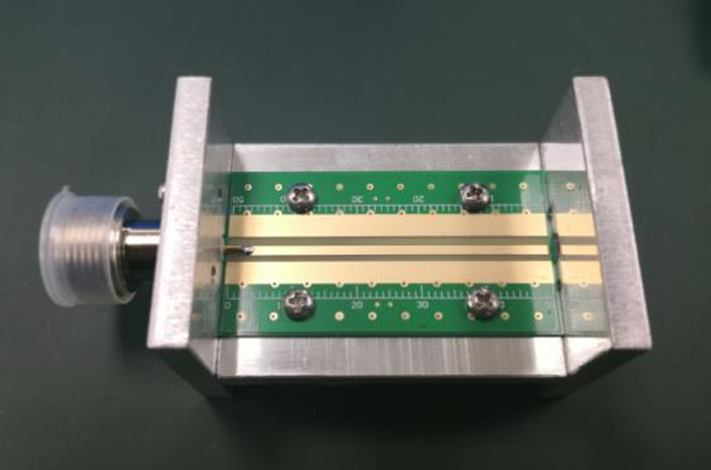
\includegraphics[width=0.75\linewidth]{figures/pe0.png} % 数字表示放缩比例
  \caption{微带开路传输线模块} % 图片标题
\end{figure}
其中微带电路参数如下：
\begin{enumerate}
  \item 工作频率2.5GHz
  \item 特性阻抗50欧姆
  \item 传输线1/2波长
  \item 微波介质基板特性：相对介电常数4.6，介质层厚度0.765mm，铜箔厚度0.035mm(1OZ)，损耗正切0.015；
\end{enumerate}

\section{实验步骤}
\subsection{开机}
打开网络分析仪电源，系统开机后需要先预热几分钟，等待仪器内器件稳定
再开始测量。观察仪器面板和测量界面（参见附2.矢量网络分析仪操作说明的第
四章快速操作入门）。
\subsection{选择测量内容}
仪器完成预热后先选择测量内容。一般先进行S参数测量。按【测量】键，
根据测试的内容选择显示面板右侧的按键，如按下[S11]软按键即测量反射，[S21]
软按键即测量传输。
\subsection{选择测量格式}
按【格式】键，可选择测量结果显示的格式，如对数幅度，史密斯圆图等。
（注意：只有在反射测量的情况下才能显示史密斯圆图）
\subsection{设置频率范围}
矢量网络分析仪扫频工作，默认最大扫描频率范围工作，如AV36580是
300KHz 扫描到3GHz。但是在具体测量的过程中，需要设置频率扫描的范围，
以便观察和得到更高精度的数据
。
以微带传输线模块测量为例，考虑到微带线设计的工作频率为2.5GHz，所

以扫描频率可暂定为2.3GHz-2.7GHz，在测量过程中也可进一步调节频率范围。
按【起始】键，然后用数字键和旁边的单位键输入测量的起始频率。此时测
量界面下方显示的起始频率变为设置值。

按【终止】键，然后用数字键和旁边的单位键输入测量的终止频率。此时测
量界面下方显示的终止频率变为设置值。
\subsection{校准}
测量校准是通过测量特性已知的标准来确定系统误差，然后在进行被测件测
量时去除这些系统误差影响的过程，通过校准可减小测量误差，提高分析仪的测
量精度。

一般情况下系统默认校准参数，为了测量更准确，每次测量之前需要连接好
射频电缆线，然后校准。

以微带传输线反射测量为例来校准。

连接射频好电缆线之后，按【校准】键，出现多个校准选项，因为反射测量
只需要用到矢网单个端口，为方便起见，可选择[机械校准]软按键，然后再选择
[单端口（反射）]。
此时显示面板右侧出现[开路器]、[短路器]和[负载]，需要用配套的校准件，
依次接上开路器、短路器和匹配负载，每接完一个校准件，就按下显示面板上相
应选项右侧的软按键，显示选项下会出现下划线，如[开路器
]，则表示按键有效。

最后按[完成单端口]软按键即完成校准，此时如果匹配负载校准件还未移除，
可看到如图显示测试界面，表示此时为史密斯圆图的匹配状态。
\begin{figure}[H]
  \centering
  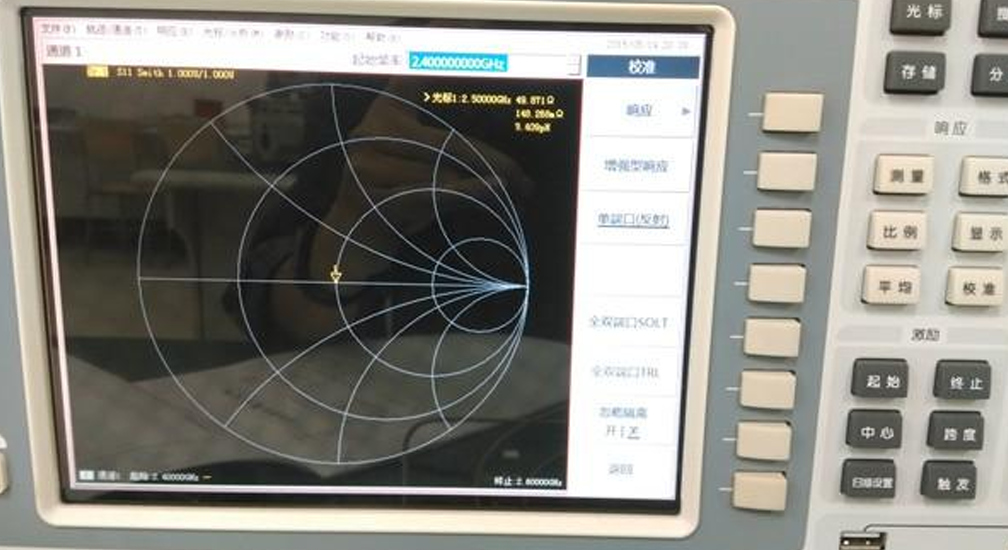
\includegraphics[width=0.75\linewidth]{figures/pe1.png} % 数字表示放缩比例
  \caption{微带开路传输线模块} % 图片标题
\end{figure}
\subsection{测量微带传输线电路模块}
在射频电缆线端接入微带开路传输线模块。然后按【光标】键打开光标，可
看到类似如图1-4的Smith曲线。旋转旋钮光标会沿着扫描曲线移动，同时可观
察右上角的测试数据。
\begin{figure}[H]
  \centering
  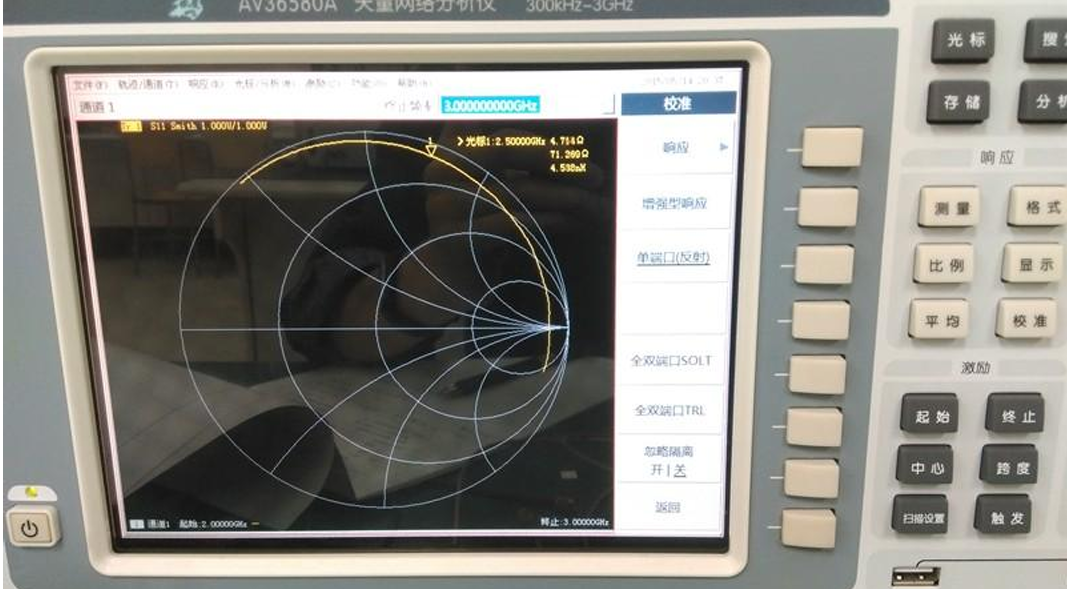
\includegraphics[width=0.75\linewidth]{figures/pe2.png} % 数字表示放缩比例
  \caption{微带开路传输线模块} % 图片标题
\end{figure}
注意：由于校准件是N接头，而很多微带传电路或模块采用的是SMA接头，
所以校准完成后需要接上N转SMA转接头才能连接电路，该转接头引起的误差
无法消除，此时测量曲线参数会有所偏移。
\subsection{其他负载测量}
参见Figure 4，以51欧姆电阻负载为例。用防静电镊子夹取一个51欧姆阻值
0805 或1206 封装的贴片电阻，放置在测量模块的微带传输线末端，将电阻两端
管脚分别架在传输线的开路端和覆铜接地端上，然后用镊子向下压紧使接触充分
有效，观察此时网络分析仪测试窗口曲线的变化即为传输线负载端接入51欧姆
电阻的情况。利用光标可观察各个频率上的反射情况。
\begin{figure}[H]
  \centering
  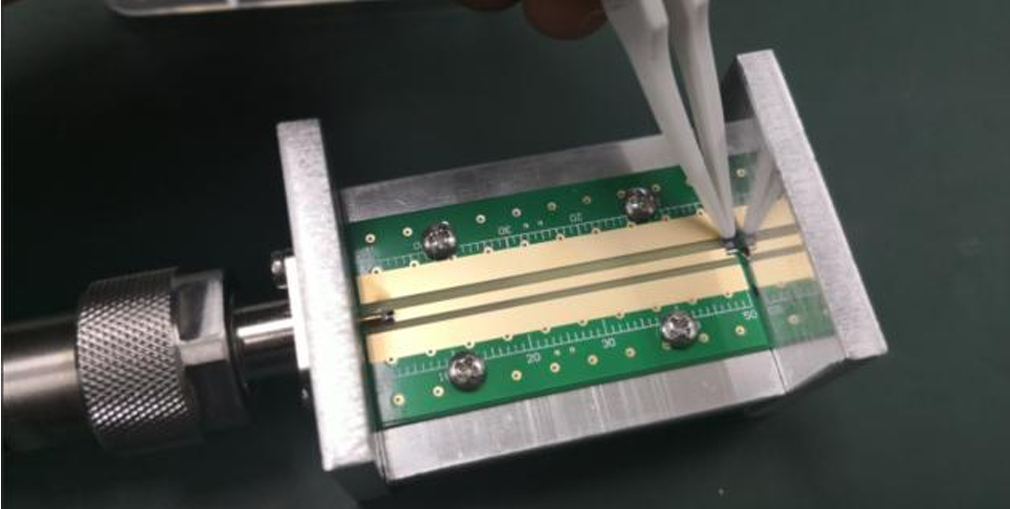
\includegraphics[width=0.75\linewidth]{figures/pe3.png} % 数字表示放缩比例
  \caption{微带开路传输线模块} % 图片标题
\end{figure}
其他负载以此类推。

实验中可测量传输线开路或短路（0欧）、匹配（49.9/51欧）电阻、1PF电
容、3.3nH电感等负载的反射特性曲线。

试计算分析微带线负载端接不同负载情况下，工作频率在2.3GHz-2.7GHz，
步进100MHz时的阻抗变化，与实验测试值对比。
\subsection{天线测量}
天线通常用网络分析仪来测试驻波比、相位等特性，用以判断该天线在工作
频段的匹配情况。本实验中，天线也可以看做一复阻抗负载，测量方法和上述负
载类似。但由于实验中的短天线为SMA接口，测量需要在微带线上焊接转换头
来连接，为方便起见将该天线直接转接在网络分析仪端口处测量，参见Figure 5。
因为此时没有用射频电缆线，所以需要对网络分析仪端口处重新进行校准操作。
\begin{figure}[H]
  \centering
  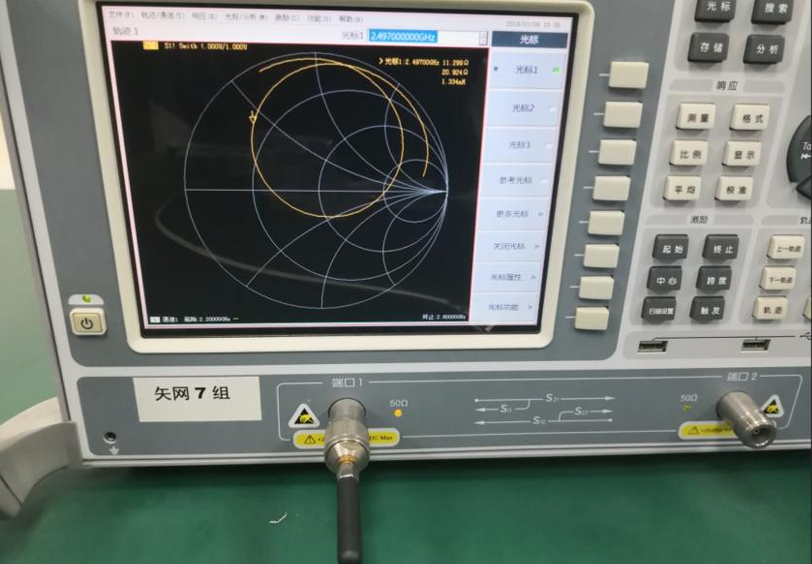
\includegraphics[width=0.75\linewidth]{figures/pe4.png} % 数字表示放缩比例
  \caption{微带开路传输线模块} % 图片标题
\end{figure}
\subsection{微带滤波器测量}
微带滤波器原理：

滤波器是体现网络特性的最好部件。本实验中以测量平行耦合线带通滤波器
网络特性为例来熟悉网络参量测量。

平行耦合线带通滤波器在微带结构中得到极为广泛的应用，其结构紧凑，适
合用平面工艺制作，寄生通带的中心频率比较高，并且在按照综合设计得到所要
求的原型滤波器参量时，有较大的结构灵活性。其结构如图Figure 6
\begin{figure}[H]
  \centering
  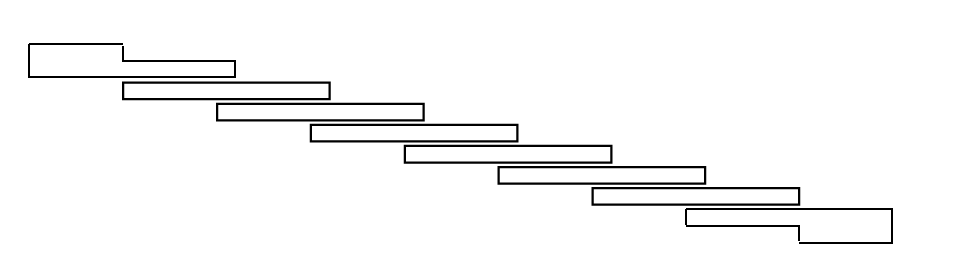
\includegraphics[width=0.75\linewidth]{figures/pe5.png} % 数字表示放缩比例
  \caption{微带开路传输线模块} % 图片标题
\end{figure}
两端开路的半波长微带线构成的谐振器相当于一LC回路，平行耦合线带通
滤波器谐振器之间的耦合是通过微带线的边缘场进行，它可用多级耦合谐振器等
效。耦合的多个LC回路具有带通特性。

由于滤波器元件的损耗对滤波性能影响较大，而作为滤波元件的耦合线段，
实际上相当于一半波偶极子天线附加反射板（即接地板），故除了导体与介质损
耗外，其辐射损耗对元件Q值下降影响也较大。在实际应用中为了改善性能，往
往需要对滤波器外加屏蔽盒。

滤波器设计已有成熟理论，平行耦合线带通滤波器设计方法可参阅《射频电
路与系统设计》。滤波器的最终性能可用网络分析仪进行测量，见图Figure 7。
\begin{figure}[H]
  \centering
  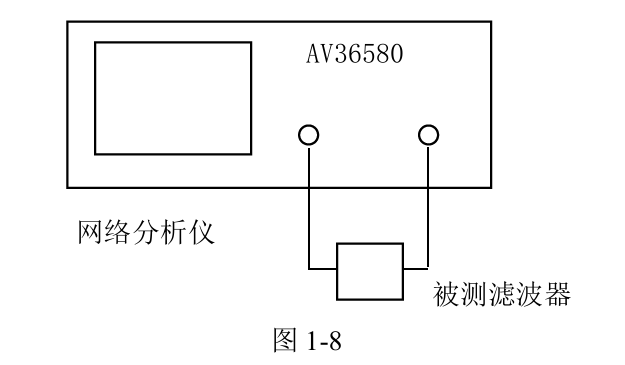
\includegraphics[width=0.75\linewidth]{figures/pe6.png} % 数字表示放缩比例
  \caption{微带开路传输线模块} % 图片标题
\end{figure}
微带滤波器测量实验步骤：

平行耦合线带通滤波器通常需要观察传输（$S_{21}$曲线）和反射（ 11
 $S_{11}$曲线）特性，其中测试反射特性步骤基本和前相同。

在测量传输特性时，需要先按【测量】键，选择[S21]软按键测量传输特性。
然后将网络分析仪两个端口都接上射频电缆和N型-SMA转接头，并用一个直通
接头将两条电缆线联通起来，然后按【校准】，选择【机械校准】->【直通响应】->【前向直通】进行直通的校准，校准成功之后，观察 21
 S曲线应该是0dB的一
条直线。此时可换上滤波器测试参数。

记录测量的结果

用手指或金属片作为外界干扰，观察滤波器特性曲线、驻波比特性和史密斯
圆图上的输入阻抗的变化。

在反射测量下，分别观察滤波器驻波比特性和史密斯圆图上的输入阻抗、反
射系数的映象。
\section{实验结果}
\subsection{记录测试数值，测试曲线可拍照贴图}
\subsubsection{分析微带传输线在不同负载下的反射特性情况，和理论计算的异同}
设传输线特性阻抗 $Z_0 = 50\,\Omega$，反射系数公式为：
\[
\Gamma = \frac{Z_L - Z_0}{Z_L + Z_0}
\]
\begin{enumerate}
  \item \textbf{传输线开路}
  \[
\Gamma_{\text{open}} = \lim_{Z_L\to\infty} \frac{Z_L - 50}{Z_L + 50} = 1
\]
\textbf{理论值}：$\Gamma_{\text{open}} = 1$
\begin{figure}[H]
  \centering
  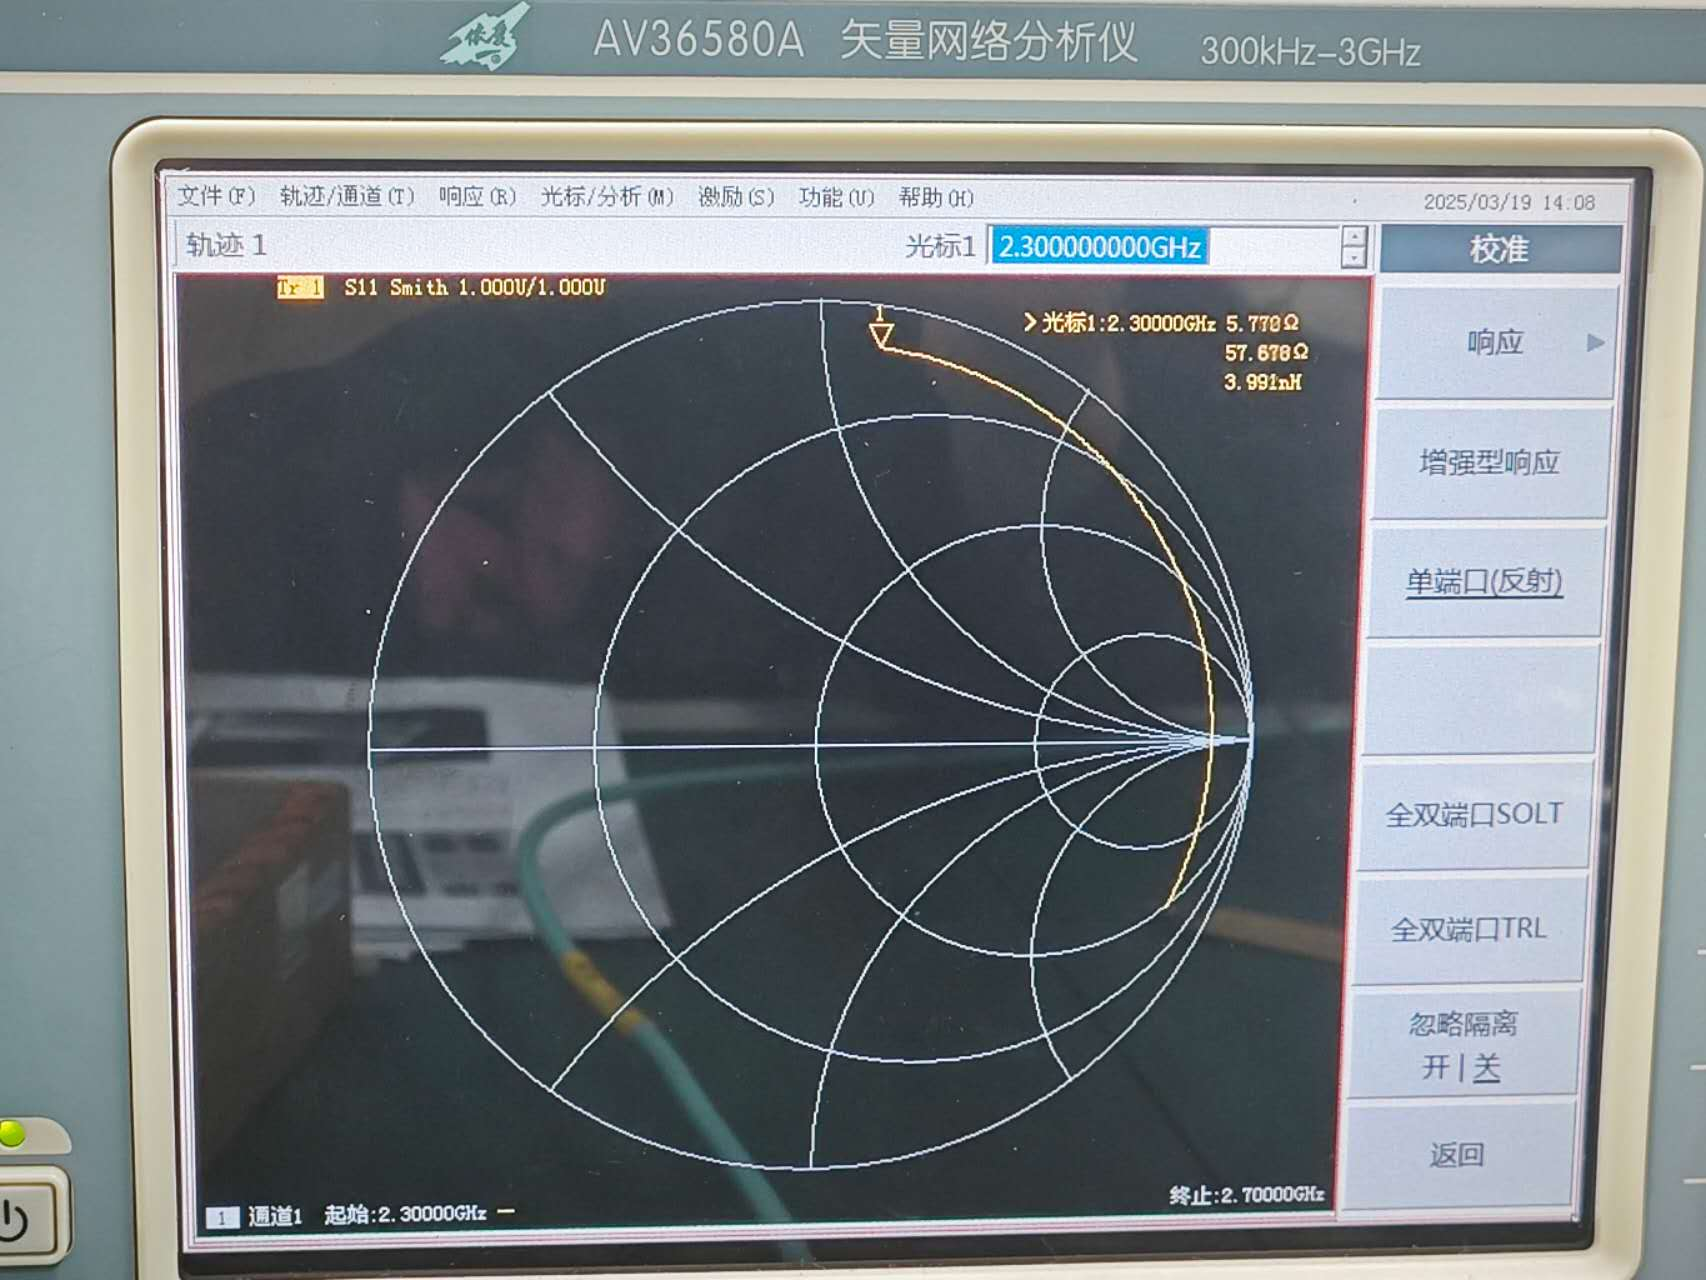
\includegraphics[width=0.75\linewidth]{figures/p10.jpg} % 数字表示放缩比例
  \caption{传输线开路图} % 图片标题
\end{figure}
\begin{table}[ht]
  \centering
  \begin{tabular}{lll}
  \toprule
  \textbf{阻抗测量值 (\si{\ohm})} & \textbf{反射系数测量值} & \textbf{反射系数理论值} \\
  \midrule
  $5.770 + j57.678$ & 
  $ 0.906 \angle 81.5^\circ$ & 
  $\Gamma=1$\\
  \bottomrule
  \end{tabular}
  \end{table}

  【分析】：对于传输线开路情况，反射系数测量幅值与理论值大致相符，
  但测量相位与理论值存在较大偏差
  \item \textbf{传输线短路}
\[
\Gamma_{\text{short}} = \frac{0 - 50}{0 + 50} = -1
\]
\textbf{理论值}：$\Gamma_{\text{short}} = -1$
  \begin{figure}[H]
    \centering
    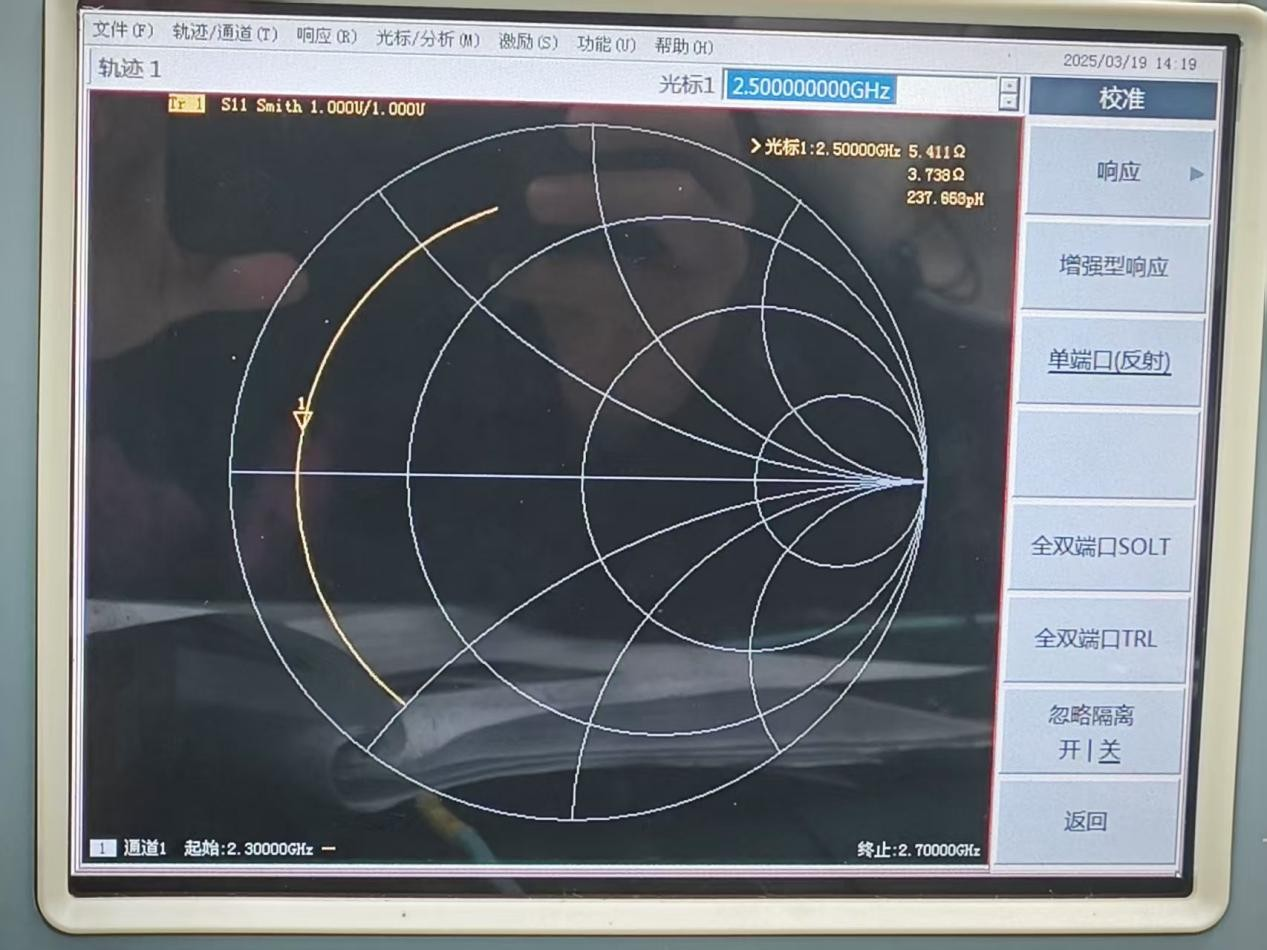
\includegraphics[width=0.75\linewidth]{figures/p13.jpg} % 数字表示放缩比例
    \caption{传输线短路图} % 图片标题
  \end{figure}
  \begin{table}[ht]
    \centering
    \begin{tabular}{lll}
    \toprule
    \textbf{阻抗测量值 (\si{\ohm})} & \textbf{反射系数测量值} & \textbf{反射系数理论值} \\
    \midrule
    $5.411 + j3.738$ & $0.806 \angle 171.3^\circ$ & $\Gamma=-1$\\
    \bottomrule
    \end{tabular}
    \end{table}
  【分析】：对于传输线短路情况，反射系数测量值与理论值大致相符，幅值误差为19.4\%，相位误差为3.9\%
  \item \textbf{负载49.9$\Omega$}
  \[
  \Gamma_{\text{match}} = \frac{49.9 - 50}{49.9 + 50} = \frac{-0.1}{99.9} \approx -0.001
  \]
\textbf{理论值}：$\Gamma_{\text{match}} \approx -0.001$
  \begin{figure}[H]
    \centering
    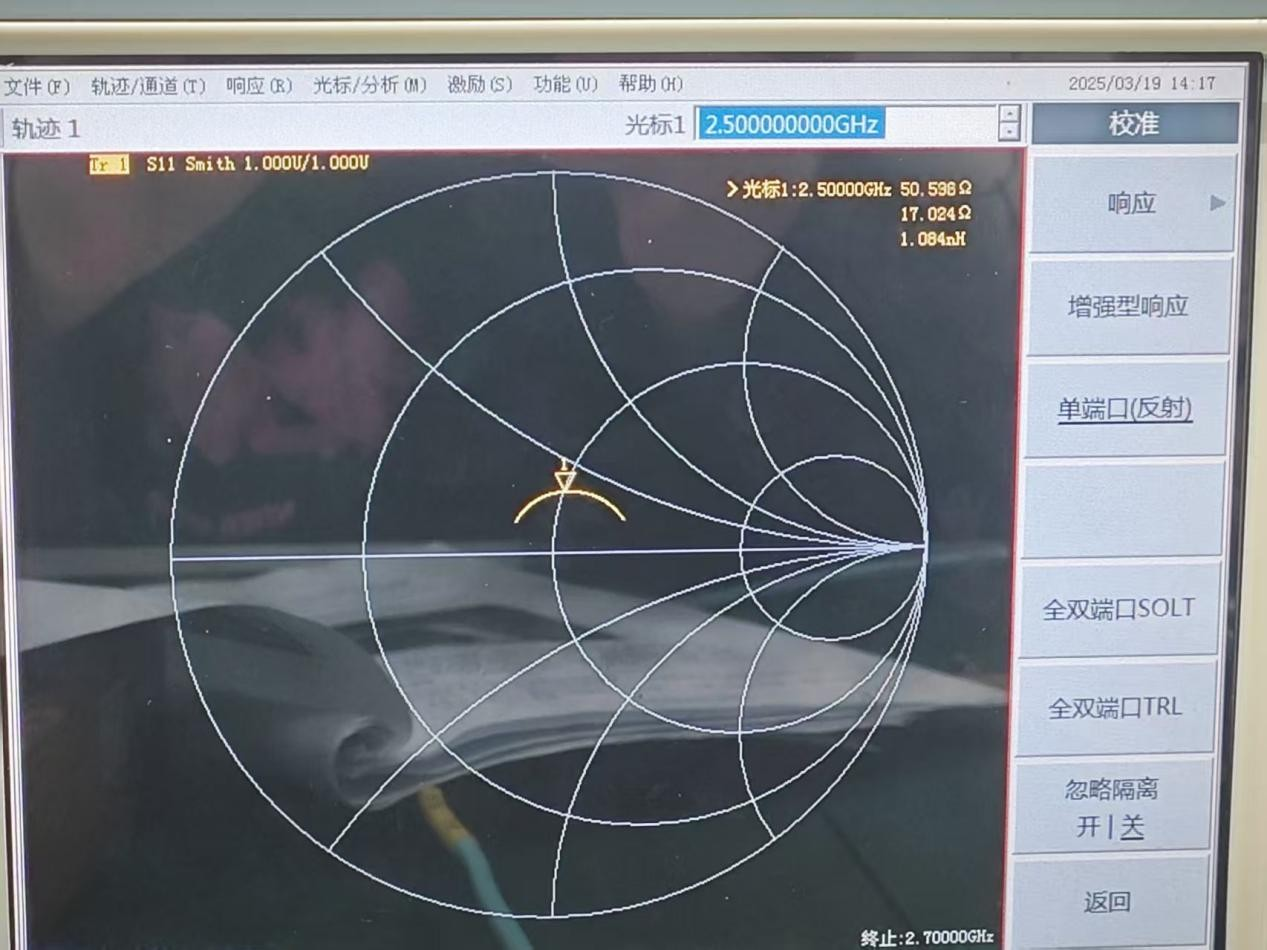
\includegraphics[width=0.75\linewidth]{figures/p11.jpg} % 数字表示放缩比例
    \caption{负载49.9$\Omega$图} % 图片标题
  \end{figure}

  \begin{table}[H]
    \centering
    \begin{tabular}{lll}
    \toprule
    \textbf{阻抗测量值 (\si{\ohm})} & \textbf{反射系数测量值} & \textbf{反射系数理论值} \\
    \midrule
    $50.598 + j17.024$ & $0.167 \angle 78.3^\circ$ & $\Gamma=-0.001$ \\
    \bottomrule
    \end{tabular}
  \end{table}
  【分析】：对于负载49.9$\Omega$情况，反射系数测量所得幅值与相位相差均较大
  \item \textbf{负载1pF电容}
  
  在$f=2.5\,\text{GHz}$时：
  \[
  Z_L = \frac{1}{j \times 2\pi \times 2.5\times10^9 \times 1\times10^{-12}} = -j63.66\,\Omega
  \]
  \[
  \Gamma_{\text{cap}} = \frac{-j63.66 - 50}{-j63.66 + 50} = \frac{-50 - j63.66}{50 - j63.66}
  \]
  \[
|\Gamma_{\text{cap}}| = 1,\quad \angle\Gamma_{\text{cap}} = -76.3^\circ
\]
\textbf{理论值}：$\Gamma_{\text{cap}} = 1\angle-76.3^\circ$
  \begin{figure}[H]
    \centering
    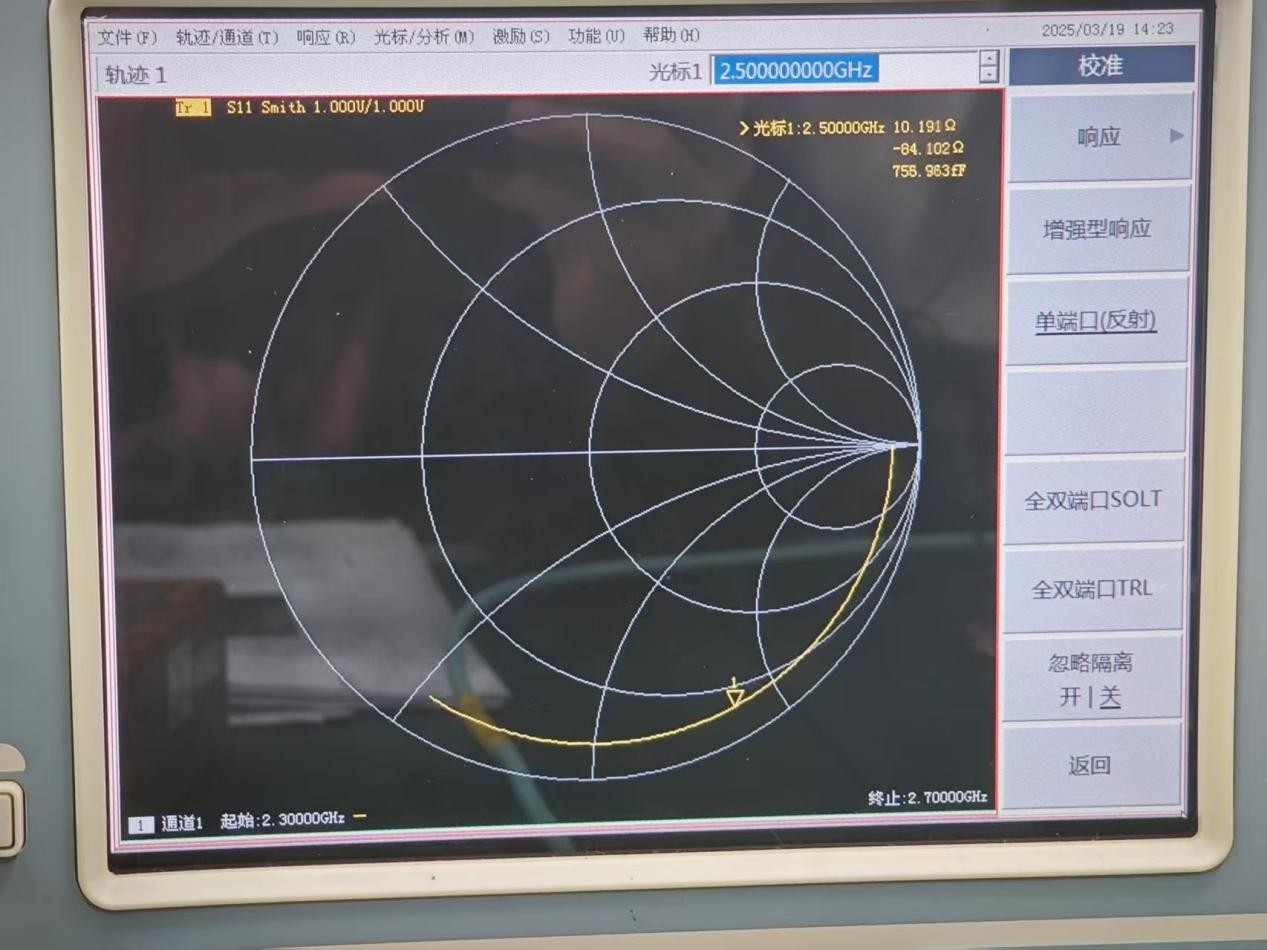
\includegraphics[width=0.75\linewidth]{figures/p12.jpg} % 数字表示放缩比例
    \caption{负载1pF电容图} % 图片标题
  \end{figure}
  \begin{table}[H]
    \centering
    \begin{tabular}{lll}
    \toprule
    \textbf{阻抗测量值 (\si{\ohm})} & \textbf{反射系数测量值} & \textbf{反射系数理论值} \\
    \midrule
    $10.191 - j84.102$ & $0.90 \angle -60.9^\circ$ & $|\Gamma|=1\angle-76.3^\circ$\\
    \bottomrule
    \end{tabular}
    \end{table}
    【分析】：对于负载1pF电容情况，反射系数测量所得幅值与相位均较接近，测得幅值相对误差为10.0\%，相位相对误差为20.2\%
  \item \textbf{负载3.3nH电感}
  
  在$f=2.5\,\text{GHz}$时：
  \[
  Z_L = j \times 2\pi \times 2.5\times10^9 \times 3.3\times10^{-9} = j51.84\,\Omega
  \]
  \[
  \Gamma_{\text{ind}} = \frac{j51.84 - 50}{j51.84 + 50} = \frac{-50 + j51.84}{50 + j51.84}
  \]
  \[
|\Gamma_{\text{ind}}| = 1,\quad \angle\Gamma_{\text{ind}} = 87.9^\circ
\]
\textbf{理论值}：$\Gamma_{\text{ind}} = 1\angle87.9^\circ$
  \begin{figure}[H]
    \centering
    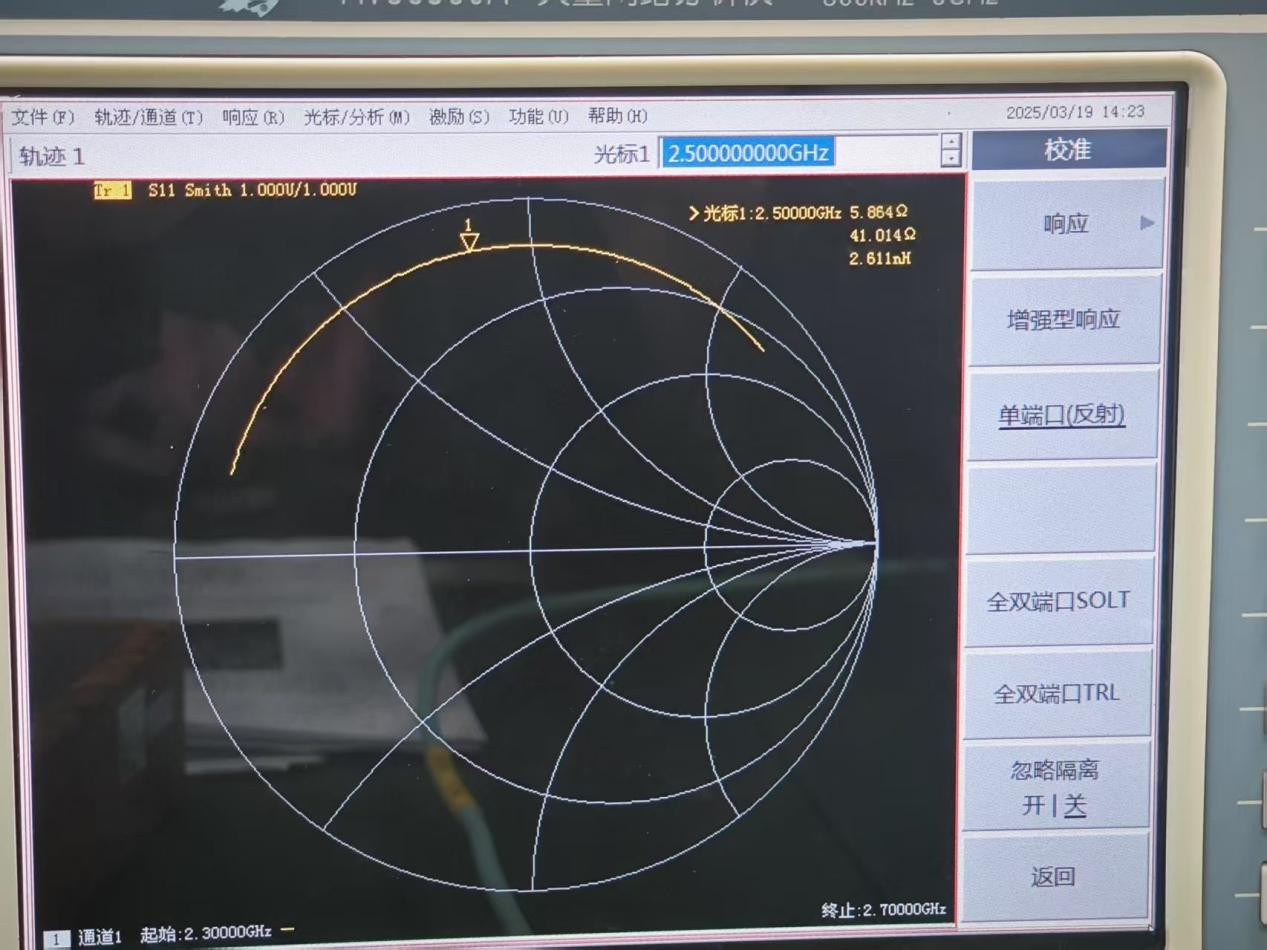
\includegraphics[width=0.75\linewidth]{figures/p14.jpg} % 数字表示放缩比例
    \caption{负载3.3nH电感图} % 图片标题
  \end{figure}
  \begin{table}[H]
    \centering
    \begin{tabular}{lll}
    \toprule
    \textbf{阻抗测量值 (\si{\ohm})} & \textbf{反射系数测量值} & \textbf{反射系数理论值} \\
    \midrule
    $5.864 + j41.014$ & $0.869 \angle 100.6^\circ$ & $|\Gamma|=1\angle87.9^\circ$ \\
    \bottomrule
    \end{tabular}
    \end{table}
    【分析】：对于负载3.3nH电感情况，反射系数测量所得幅值与相位均较接近，测得幅值相对误差为13.1\%，相位相对误差为14.4\%
    \item \textbf{误差分析}
      \begin{itemize}
        \item 由于传输线自身损耗，实验数据会总体向负载端移动，传输线开路时没有与史密斯圆图的最外圈完全重合
        \item 由于实验所用的电子元件非焊接，而是用镊子压在模型上的，存在一定误差
        \item 
      \end{itemize}
    
  \end{enumerate}

\subsubsection{分析天线的驻波比特性曲线}

\begin{figure}[H]
  \centering
  \begin{minipage}[b]{0.5\linewidth}
      \centering
      \includegraphics[width=0.9\textwidth]{figures/P22.jpg}
      \caption{天线对数幅度曲线}
  \end{minipage}%
  \begin{minipage}[b]{0.5\linewidth}
      \centering
      \includegraphics[width=0.9\textwidth]{figures/P23.jpg}
      \caption{天线驻波比曲线}
  \end{minipage}
\end{figure}

【分析】：从天线的对数幅度曲线与天线驻波比曲线中可以看出，在1.68GHz情况下，对数幅度有最小值-22.736dB<-14dB，驻波比有最小值1.153<1.5，
理想情况下，天线驻波比等于1，说明传输给天线的电磁波全部发送出去，而一般要求天线驻波比小于1.5，故该天线符合设计要求
\subsubsection{分析测量的微带耦合滤波器的滤波特性，试说明设计优劣情况}
\begin{figure}[H]
  \centering
  \begin{minipage}[b]{0.5\linewidth}
      \centering
      \includegraphics[width=0.9\textwidth]{figures/P31.jpg}
      \caption{微带耦合滤波器的滤波特性1}
  \end{minipage}%
  \begin{minipage}[b]{0.5\linewidth}
      \centering
      \includegraphics[width=0.9\textwidth]{figures/P32.jpg}
      \caption{微带耦合滤波器的滤波特性2}
  \end{minipage}
\end{figure}
【分析】：根据滤波器曲线，读出中心频率 \( f_0 = 2.392\ \mathrm{GHz} \)，对应 \( -8.030\ \mathrm{dB} \)；在中心频率 \( -300\ \mathrm{MHz} \) 处，对应 \( -45.909\ \mathrm{dB} \)；在中心频率 \( +300\ \mathrm{MHz} \) 处，对应 \( -42.393\ \mathrm{dB} \)。

综上可以得到滤波器的部分特性：

\begin{table}[H]
  \centering
  \begin{tabular}{ll}
      \toprule
      \textbf{滤波器参数} & \textbf{数值} \\
      \midrule
      3dB 带宽 & $207.904\ \si{MHz}$ \\
      插入损耗 & $-6.751\ \si{dB}$ \\
      中心频率 & $2.392\ \si{GHz}$ \\
      带内纹波 & $\approx 0$ \\
      阻带衰减 & $-45.909\ \si{dB}$ -- $-42.393\ \si{dB}$ \\
      \bottomrule
  \end{tabular}
\end{table}

该滤波器为带通滤波器，带宽较小，需优化，但在中心频率附近线性度良好，带内纹波小、失真低，整体滤波性能达标。

【注】：测量时发现曲线形状有点“平顶”，询问老师后得知要重新校准，而仔细重新校准后仍然如图，怀疑是滤波器问题

下为$S-\omega$ 关系曲线：

\begin{figure}[H]
  \centering
  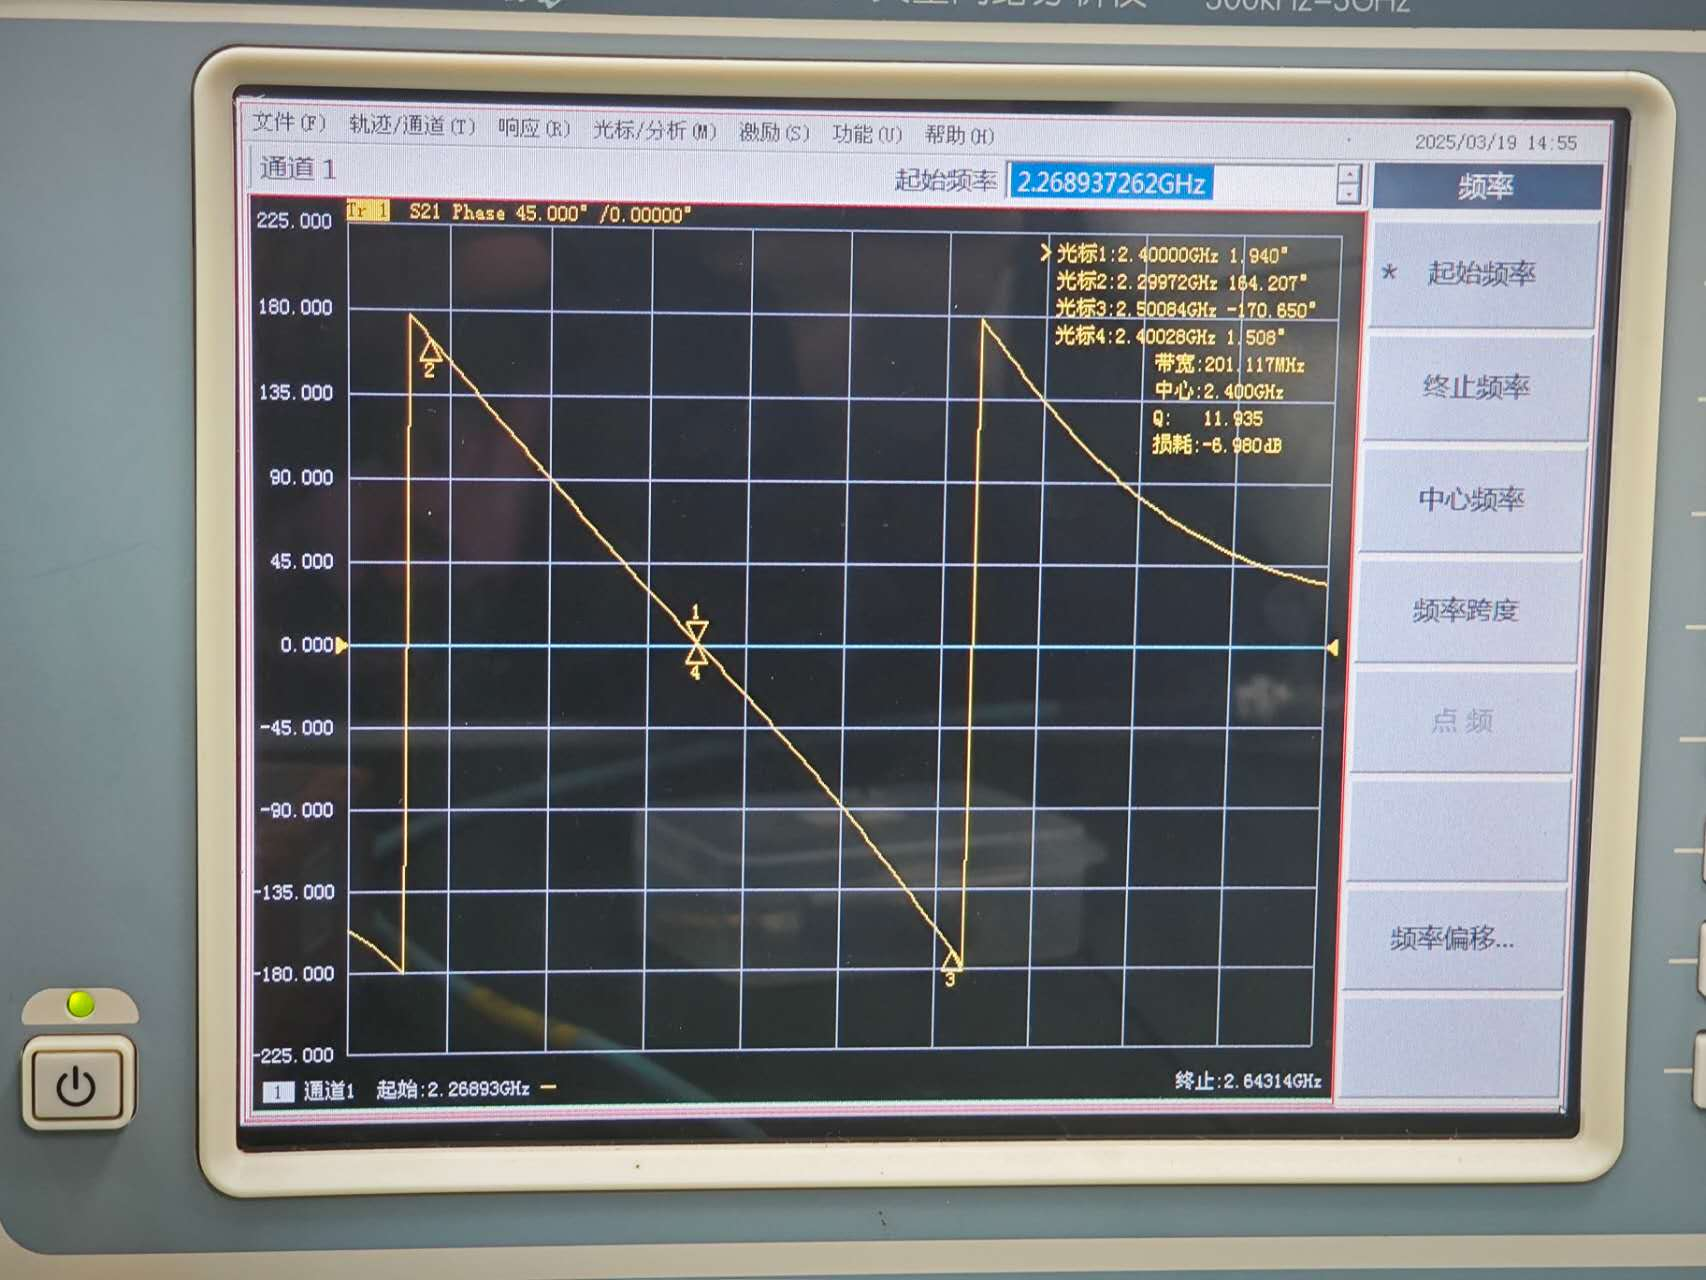
\includegraphics[width=0.75\linewidth]{figures/p39.jpg} % 数字表示放缩比例
  \caption{$S-\omega$ 关系曲线} % 图片标题
\end{figure}

\subsection{思考题}
\subsubsection{什么是S参数?}
S参数（散射参数）用于描述射频（RF）和微波网络中信号的反射、传输和散射特性。
它们主要包括四个参数：S11、S12、S21和S22。
\begin{itemize}
  \item \textbf{S11}：端口1的反射系数
  \item \textbf{S12}：从端口2到端口1的反向传输系数
  \item \textbf{S21}：从端口1到端口2的正向传输系数
  \item \textbf{S22}：端口2的反射系数
\end{itemize}

\subsubsection{如果不校准，直接接入射频电缆和电路模块测量会对结果有什么影响，为什么？}
若不校准直接测量，系统误差（如电缆损耗、连接器反射、仪器内部噪声）会被引入结果，
造成测得的S参数，插入损耗等数据不准确
\subsubsection{如何测量转接头对测试曲线的影响?}
连接转接头，测量其S参数（如S11、S21）。
分析测得的插入损耗、反射系数等参数，与未连接时进行对比，量化转接头对信号的衰减和相位偏移影响
\subsubsection{利用实验内容2中已知的设计参数，计算50欧半波长微带线的长度和宽度。}
\begin{itemize}
  \item 相对介电常数：$\epsilon_r = 4.6$
  \item 介质厚度：$h = 0.765\,\text{mm}$
  \item 铜箔厚度：$t = 0.035\,\text{mm}$
\end{itemize}

\begin{align*}
  B &= \frac{377\pi}{2Z_0\sqrt{\epsilon_r}} \\
    &= \frac{377 \times 3.1416}{2 \times 50 \times \sqrt{4.6}} \\
    &\approx 5.526
\end{align*}

\begin{align*}
  W &= \frac{2h}{\pi}\left[B - 1 - \ln(2B - 1) + \frac{\epsilon_r - 1}{2\epsilon_r}\left(\ln(B - 1) + 0.39 - \frac{0.61}{\epsilon_r}\right)\right] \\
    &\approx 1.41\,\text{mm}
\end{align*}

\begin{equation*}
  \epsilon_{\text{eff}} = \frac{\epsilon_r + 1}{2} + \frac{\epsilon_r - 1}{2}\left(1 + \frac{12h}{W}\right)^{-0.5} \approx 3.457
\end{equation*}

\begin{equation*}
  L = \frac{c}{2f\sqrt{\epsilon_{\text{eff}}}} = \frac{3 \times 10^8}{2 \times 2.5 \times 10^9 \times \sqrt{3.457}} \approx 32.28\,\text{mm}
\end{equation*}

\begin{itemize}
  \item 微带线宽度：$W \approx 1.41\,\text{mm}$
  \item 半波长长度：$L \approx 32.28\,\text{mm}$
\end{itemize}

\subsection{实验的收获与体会}
\begin{itemize}
  \item 掌握了矢量网络分析仪的使用：通过实际操作，熟悉了S参数的测量方法，特别是反射和传输特性。
  \item 理解了微带传输线的特性：通过不同负载下的反射特性测量，体会到负载对信号传输的影响。
  \item 学会了如何进行仪器校准：明白了如何通过仪器校准，确保测试结果的准确性。
\end{itemize}

\subsection{实验的建议与意见}
\begin{itemize}
  \item 建议在实验前加强对矢量网络分析仪等仪器的具体操作讲解
  \item 建议与理论课对接，融实践于理论，否则很多内容操作的云里雾里的
\end{itemize}
\end{document}
